% vim: ft=tex
%!TEX root=ast2016.tex

% GRAPHIC: This is the box and whisker plot that shows the mutation score for the two techniques
%!TEX root=ast2016.tex

\begin{figure*}[t]
  \centering
  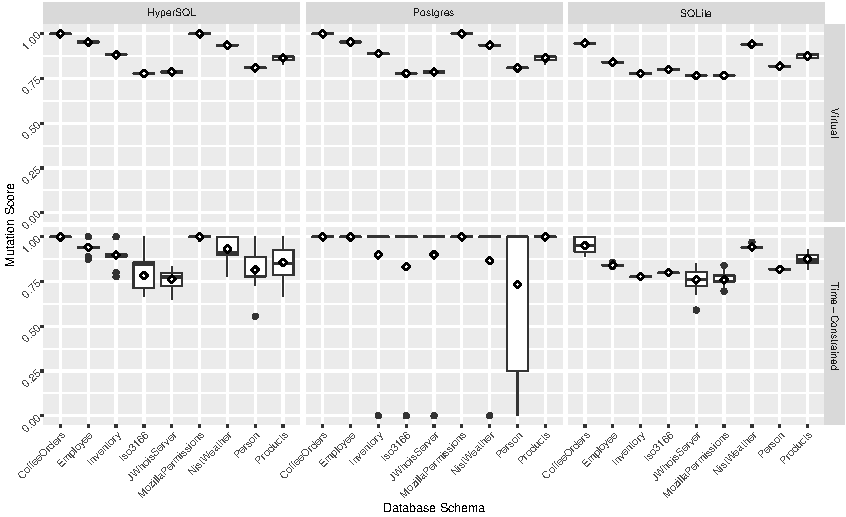
\includegraphics[scale=1.0]{graphics/graphic_bwplot_schema_mutationscore_vm_tcm.pdf}
  \caption{Box plot of the mutation score for the virtual and time-constrained mutation analysis techniques.}\label{fig:graphic_bwplot_schema_mutationscore_vm_tcm}

  % NOTE: This caption is not yet correct.

  {\small \justifying{\noindent The meaning for this box plot's elements is the same as the meaning of those described
      in the subcaption of Figure~\ref{fig:graphic_bwplot_schema_analysistime_org_vm}. Additionally, in this box plot a
      filled circle denotes an outlier and the open diamond is the mean value. Using test suites from thirty separate
      runs of the search-based test data generation method developed by McMinn \etal~\cite{McMinn2015}, this plot shows
      the variation in the mutation score for both the virtual and the time-constrained method and for all of the chosen
  relational schemas and the three database management systems. } \par}

\end{figure*}


% GRAPHIC: This is the bar chart of the number of mutants that each technique ran during mutation analysis
% NOTE: This graph was removed due to space constraints, it can be summarized in the text, I think.
% %!TEX root=ast2016.tex

\begin{figure*}[t]
  \centering
  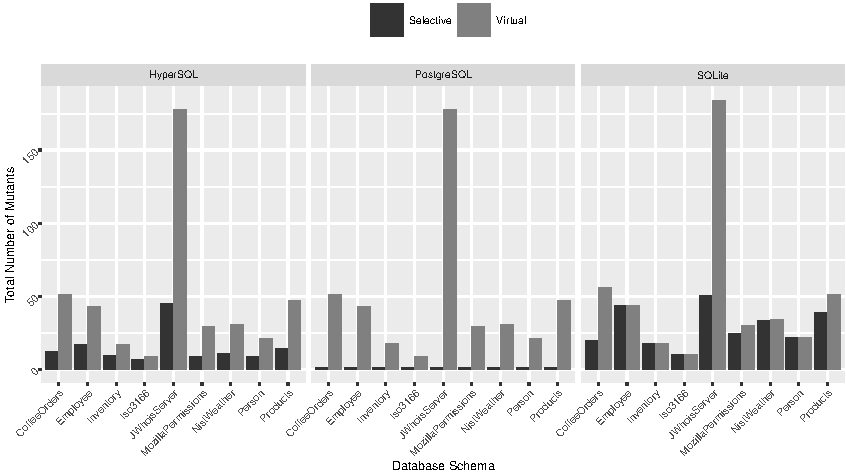
\includegraphics[scale=1.0]{graphics/graphic_barplot_schema_mutantcount_vm_tcm.pdf}
  \caption{Bar plot of the mutant count for both the virtual and time-constrained mutation analysis techniques.}
  \label{fig:graphic_barplot_schema_mutantcount_vm_tcm}

  {\small \justifying{ \noindent In this plot the height of the bar corresponds to the number of mutants subject to
      analysis by the virtual and time-constrained methods; this count is reported for all of the chosen relational
      schemas and the three database management systems. Since the time-constrained technique employs randomness to
      select mutants that can be run within a specified time limit, the height of a light grey bar is the average across
      a total of thirty runs; virtual mutation analysis is deterministic and thus the height of the dark grey bar is a
      direct count. } \par}

\end{figure*}


\inlineheading{Virtual and Time-Constrained Mutation} Since the experiments revealed that \vma~is faster than the
\Original~one in $22$ out of the $27$ studied configurations --- and competitive with the DBMS-based method in the other
$5$ --- it is important to ascertain whether the presented technique might yield accurate mutation scores in some
circumstances. To this end, Figure~\ref{fig:graphic_bwplot_schema_mutationscore_vm_tcm} presents the mutation score of
the virtual approach and a time-constrained method in which \Original~is only allowed to run for as long as virtual.





